% Template adapted from the Eurographics SGP 2016 template

\documentclass{6838publ}
\usepackage{6838}

\SpecialIssuePaper
\electronicVersion 
\ifpdf \usepackage[pdftex]{graphicx} \pdfcompresslevel=9
\else \usepackage[dvips]{graphicx} \fi

\PrintedOrElectronic

\usepackage{t1enc,dfadobe}
\usepackage{egweblnk}
\usepackage{cite}
\usepackage{lipsum}
\usepackage{amsmath}
\usepackage{amsfonts}

\title[Shortened title]{Paper Title}

\author[J.\ Solomon \& C.F.\ Gau\ss]
       {Justin Solomon$^1$
        and Carl Friedrich Gau\ss$^{2}$
        \\
         $^1$MIT Department of Electrical Engineering and Computer Science\\
         $^2$Department of Astronomy, Universit\"atssternwarte G\"ottingen
       }

\begin{document}

\teaser{
 
\includegraphics[width=.75\linewidth]{cat_wide}
 \centering
  \caption{An optional teaser figure at the top of your paper can help readers quickly understand what your work is about.}
\label{fig:teaser}
}

\maketitle

\begin{abstract}
The abstract includes a few sentences describing the project, including the motivation, technical approach, and results. \lipsum[1]
\end{abstract}

\section{Introduction}

A few paragraphs with an intuitive/accessible description of the motivation for your project.  What is new?  What are the applications?

\section{Related Work}

% Descriptions of and citations to academic research papers and/or existing software products related to your work.  Here is an example of how to cite a paper~\cite{solomon-2016}; see \texttt{6838bibsample.bib} for bibliography entries.

\cite{alvarez-melisGromovWassersteinAlignmentWord2018}

\section{Technical Approach}\label{sec:technical_approach}

\begin{figure}[t]
\centering
 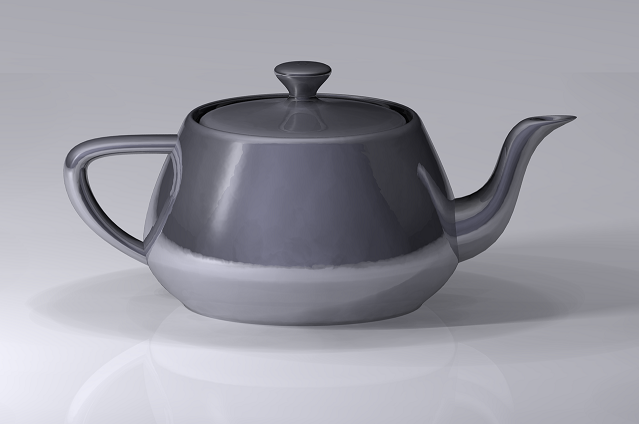
\includegraphics[width=.75\linewidth]{teapot}
\caption{This is an example of a single-column figure.}\label{fig:teapot}
\end{figure}

A description in words, equations, algorithm listings, and/or flow charts describing your approach.  

Some useful \LaTeX\ tips:  Inline equations are useful for small expressions, like $E=mc^2$.  Unnumbered equations can take up more space:
$$\int_\Omega \nabla\cdot F\,dV= \oint_{\partial\Omega} F\cdot\hat n\,dA.$$
If you need a number in an equation, you can do that as follows:
\begin{equation}\label{eq:green}
\int_U (\varphi\Delta\psi + \nabla\varphi\cdot\nabla\varphi)\,dV=\oint_{\partial U}\psi(\nabla\varphi\cdot\hat n)\,dA.
\end{equation}
Then you can refer to equation numbers like~\eqref{eq:green}.  If you use \texttt{label}, you can refer to other items, like sections \S\ref{sec:technical_approach} and figures, e.g.\ Figure~\ref{fig:teapot}.  Never hard-code the number of a section, equation, or figure!

\section{Results}

Figures/tables illustrating the results of your work, as well as text interpreting these results.

\bibliographystyle{eg-alpha-doi}
\bibliography{optimal_transport}

\end{document}
